
% ----------------------------- %
% Section 1
% ----------------------------- %
\section*{How Can We Solve This Problem?}

Since this problem is on Chapter 8.5: 
\textit{Integration of Rational Functions
by Partial Fractions}, I thought we'd
have to use an integration technique
involving partial fractions, which we will
learn in \textit{Lesson 14}. However,
since we haven't learned about partial fractions
yet - as of June 28, 2022 - I learned
by trial and error that this problem can be 
solved by using u-substitution.

% ----------------------------- %
% Section 2
% ----------------------------- %
\section*{Solution}
 
Let's start backwards. Here's the solution:

\begin{equation}
\textbf{41.}\quad \int \frac{cosy}{sin^2y+siny-6} dy =	
	\frac{2}{\sqrt{23}} tan^{-1}\bigg(
		\frac{2}{\sqrt{23}}\big(
			siny+\frac{1}{2}
		\big)
	\bigg) + C
\end{equation}

As you can see, the integral - or the solution - of 
this problem is in the form of $ tan^{-1}x + C $. 
This is because it turns out that the problem can be 
rewritten in what we learned in \textit{Lesson 5} 
as the integrand of an inverse trigonometric function. 
We learned in \textit{Lesson 5} that if we differentiate
an inverse trigonometric function like $ tan^{-1}x $,
we get $ \frac{1}{1+x^2} $. In other words,
$ \frac{d}{dx}\left( \tan^{-1}x \right) = \frac{1}{1+x^2} $.
Now, what this means is that $ \tan^{-1}x $ should also be the
integral of $ \frac{1}{1+x^2} $. 

This is the reason why the following equation, which I got
from from \textit{Lesson 5}, holds true:

\begin{equation}
\int \frac{1}{a^2+u^2} du = 
	\frac{1}{a}\tan^{-1}(\frac{u}{a}) + C
\end{equation}

Now, let's go back to our problem. What we'll see is
that $\textbf{41.}\ \int \frac{cosy}{sin^2y+siny-6} dy $
can be rewritten with u-substitution and with completing
the square. It can eventually be rewritten in the form of 
$ \int \frac{1}{1+u^2} du $; hence, the solution is in the
form of $ tan^{-1}u + C $.
	 
% ----------------------------- %
% Section 3
% ----------------------------- %
\section*{Steps}
	 
Let's do u-substitution and complete the square:
\begin{flalign*}
	\textbf{41.}\quad \int \frac{cosy}{sin^2y+siny-6} dy 
	&= \int \frac{cosy}{u^2+u+6}dy
	& & & (u = siny) \\[1ex]
	&= \int \frac{cosy}{u^2+u+6} \cdot \frac{du}{cosy}
	& & & (dy = \frac{du}{cosy}) \\[1ex]
	&= \int \frac{1}{u^2+u+6} du \\[1ex]
	&= \int \frac{1}{(u+\frac{1}{2})^2+\frac{23}{4}} du
	& & & (\text{completing the square}) \\[1ex]
	&= \int \frac{1}{w^2+\frac{23}{4}} du
	& & & (w = u+\frac{1}{2}) \\[1ex]
	&= \int \frac{1}{w^2+\frac{23}{4}} dw
	& & & (du = dw) \\[1ex]	
	&= \int \frac{1}{\frac{23}{4}(\frac{4}{23}w^2+1)} dw
	& & & (\text{algebraically rewriting}) \\[1ex]
	&= \int \frac{4}{23} \cdot \frac{1}{\frac{4}{23}w^2+1} dw \\[1ex]	
	&= \frac{4}{23}\int \frac{1}{\frac{4}{23}w^2+1} dw \\[1ex]	
	&= \frac{4}{23}\int \frac{1}{z^2+1} dw	
	& & & (z = \frac{2}{\sqrt{23}}w) \\[1ex]
	&= \frac{4}{23}\int \frac{1}{z^2+1} \cdot \frac{\sqrt{23}}{2} dz	
	& & & (dw = \frac{\sqrt{23}}{2}dz) \\[1ex]
	&= \frac{4}{23} \cdot \frac{\sqrt{23}}{2} \int \frac{1}{z^2+1} dz \\[1ex]	
	&= 2 \cdot \frac{23^{\frac{1}{2}}}{23^{1}} \int \frac{1}{z^2+1} dz \\[1ex]	
	&= 2 \cdot 23^{\frac{1}{2}-1} \int \frac{1}{z^2+1} dz \\[1ex]
	&= 2 \cdot 23^{-\frac{1}{2}} \int \frac{1}{z^2+1} dz \\[1ex]
	&= \frac{2}{\sqrt{23}} \int \frac{1}{z^2+1} dz \\[1ex]
	&= \frac{2}{\sqrt{23}} tan^{-1}z + C 
	& & & \bigg(\int \frac{1}{a^2+u^2} du = 
	\frac{1}{a}\tan^{-1}(\frac{u}{a}) + C\bigg)
\end{flalign*}

\newpage
Finally, we can substitute back $ u = siny $, $ w = u + \frac{1}{2} $,
and $ z = \frac{2}{\sqrt{23}} $.
\begin{align*}
	\textbf{41.}\quad \int \frac{cosy}{sin^2y+siny-6} dy 
	&= \frac{2}{\sqrt{23}} tan^{-1}z + C \\
	&= \frac{2}{\sqrt{23}} tan^{-1}\bigg(
		\frac{2}{\sqrt{23}}w
	\bigg) + C \\
	&= \frac{2}{\sqrt{23}} tan^{-1}\bigg(
		\frac{2}{\sqrt{23}}\big(
			u+\frac{1}{2}
		\big)
	\bigg) + C \\
	&= \frac{2}{\sqrt{23}} tan^{-1}\bigg(
		\frac{2}{\sqrt{23}}\big(
			siny+\frac{1}{2}
		\big)
	\bigg) + C
\end{align*}
	
% ----------------------------- %
% Section 4
% ----------------------------- %
\section*{Geometrically Verifying the Integral}



\newpage
You can insert Jupyter Lab style code blocks.
First, write your code on Jupyter Lab, export it as LaTeX
by clicking \inlinecode{File}, \inlinecode{Export ... As},
and \inlinecode{LaTeX}.

When you export your Jupyter Lab file into a \LaTeX file,
you'll see a lot of preambles on the top. These preambles
are what makes the code cells look 
the way they do. You don't
need to copy any of those preambles because they have already
been cloned into \inlinecode{coding.tex} and are
automatically loaded by \inlinecode{main.tex}. 
Anyway, skip to the bottom of the exported file, where
your code parts are. Your codes will start with
\inlinecode{\\begin\{tcolorbox\}} and end with \inlinecode{\\end\{Verbatim\}}.

Copy and paste these into anywhere on \inlinecode{body.tex}.
Now, when you compile \inlinecode{main.tex}, every content
on \inlinecode{body.tex} - including your codes - will render like this example pdf.

    \begin{tcolorbox}[breakable, size=fbox, boxrule=1pt, pad at break*=1mm,colback=cellbackground, colframe=cellborder]
\prompt{In}{incolor}{3}{\boxspacing}
\begin{Verbatim}[commandchars=\\\{\}]
\PY{c+c1}{\PYZsh{} Comments}
\PY{n+nb}{print}\PY{p}{(}\PY{l+s+s1}{\PYZsq{}}\PY{l+s+s1}{Hello world}\PY{l+s+s1}{\PYZsq{}}\PY{p}{)}
\end{Verbatim}
\end{tcolorbox}

    \begin{Verbatim}[commandchars=\\\{\}]
Hello world
    \end{Verbatim}

\section*{Inserting Inline Codes}
\noindent You can insert inline code with
\inlinecode{\textbackslash{}inlinecode\{...\}}.

% ----------------------------- %
% Author Guidelines
% ----------------------------- %
\section{General Guidelines}

\noindent Please read these instructions carefully.   The objective of this template is to enable you in an easy way to style your article attractively in a style similar to that of the typeset journal. It should be emphasized, however, that the final appearance of your paper in print and in electronic media may likely vary to some extent from the presentation achieved in this template.
    

\begin{equation}\label{eqn:quad}
x = \frac{-b \pm \sqrt{b^2 - 4ac}}{2a}
\end{equation}
  
has all non-zero principle minors, $A_1, A_2$ and $A_3$.  Therefore,  there is a unique LU factorization with both $L$ and $U$ nonsingular given by 

% ----------------------------- %
% Math: Theorems/Defs
% ----------------------------- %
\section{Definition, Theorem, Corollary}


\begin{definition}
Definitions are if and only if statements.  
\end{definition}

\begin{verbatim}
\begin{definition}
Definitions are if and only if statements.  
\end{definition}
\end{verbatim}

%: THEOREM: Infinite LU Factorizations
\begin{theorem}[Matrices with Infinitely Many LU Factorizations]
{For $A \in M_n$, if two or more of any first $(n-1)$ columns are linearly dependent or any of the first $(n-1)$ columns are 0, then $A$ has infinitely many LU factorizations.}
\end{theorem}

%: proof
\begin{proof} We will prove only for the the case when $A \in M_3$. \\
 \begin{align} 
&dm + r = e  \Rightarrow r = e-dm \label{eqn:1}\\
&dn + rp = f \Rightarrow p=\frac{f-dn}{r} \label{eqn:2}\\
&gm + s = h \Rightarrow s = h - gm \label{eqn:3}\\
&gn + sp + t = i \Rightarrow t  = i-sp-gn \label{eqn:4}
\end{align}
 
\end{proof} % end proof
 

% Corollary
\begin{corollary}
If $x$, then $y$.
\end{corollary}



% ----------------------------- %
% Examples
% ----------------------------- %
\section{Examples}\label{ex:x1}
Here is an example of an example.


\begin{example}
Let  $\{1,2,3\}$ and $\{2,1,3\}$ be two lists of integers.  Then, to check if the two lists are equal we would have,   
	\begin{center}
		\texttt{ \{1,2,3\} == \{2,1,3\} }.
	\end{center}\label{ex:equallists}
\end{example}


\begin{verbatim}
\begin{example}
Let  $\{1,2,3\}$ and $\{2,1,3\}$ be two lists of integers.  Then, to check if the two lists are equal we would have,   
	\begin{center}
		\texttt{ \{1,2,3\} == \{2,1,3\} }.
	\end{center}\label{ex:equallists}
\end{example}
\end{verbatim}

% ----------------------------- %
% Figures
% ----------------------------- %
 \subsection*{Figures}
Figures should be high quality (1200 dpi for line art, 600 dpi for grayscale and 300 dpi for color, at the correct size). The preferred method of including graphics in the \textit{North American GeoGebra Journal} is to export to TiKz. Other acceptable file formats include: EPS, PS, PNG, JPEG, or TIFF.  
  
 \begin{figure}[h!] %  figure placement
    \centering
    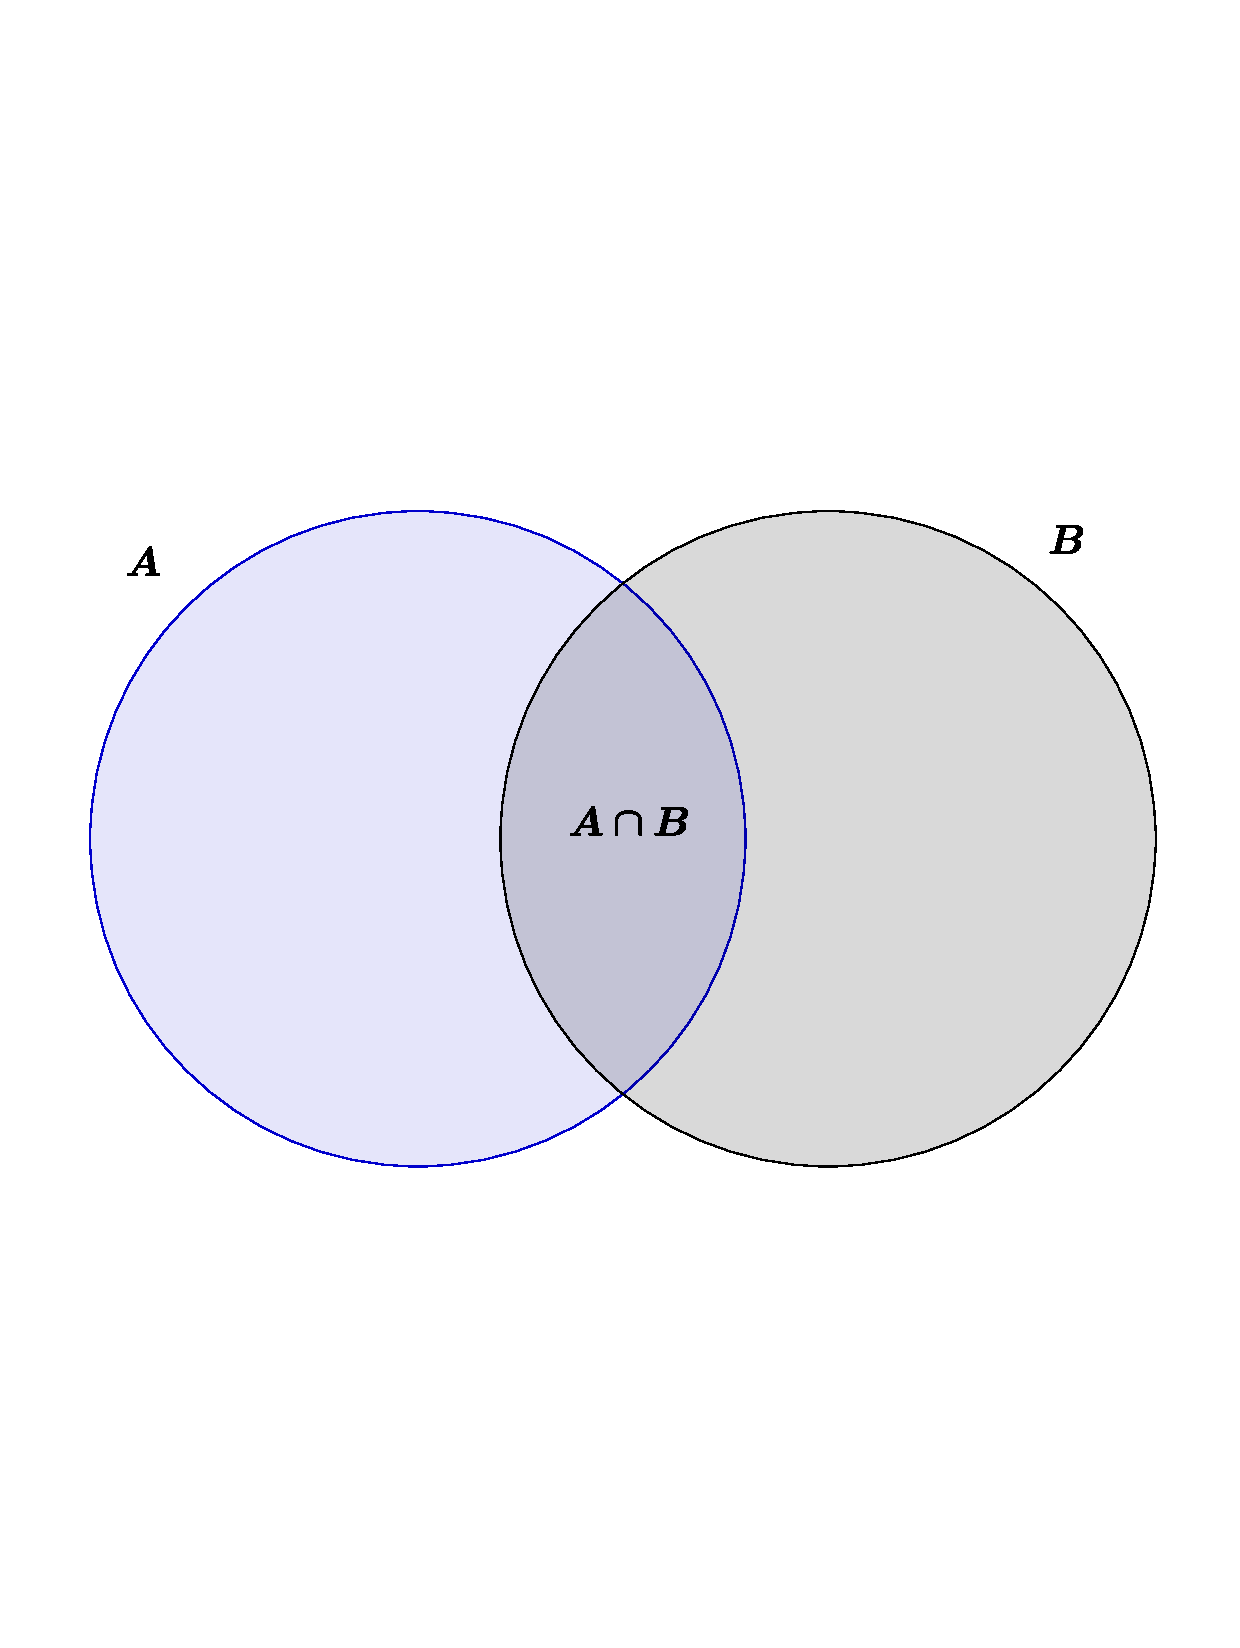
\includegraphics[scale=0.5]{figs/venn.pdf} 
    \caption{Provide a short caption description.}
    \label{fig:number}
 \end{figure}
 
